\documentclass[sumlimits, intlimits]{beamer}

\usepackage[utf8]{inputenc}
\usepackage[T1]{fontenc}
\usepackage[english]{babel}
\usepackage{hyperref}
\usepackage{lmodern, microtype}
\usepackage[margin=2cm]{caption}
\usepackage{booktabs}
\usepackage{graphicx}

\usepackage{amsfonts, amsmath, amssymb}
\usepackage{mathtools}
\newcommand \twopi{{{\scriptstyle(2}\mskip-2.0mu\pi{\scriptstyle)}}}
\newcommand \ee{{\mathrm e}}
\newcommand \ii{{\mathrm i}}
\newcommand \full{{\mathrm d}}
\newcommand \fulld[1]{{\frac \full{\full {#1}}}}
\newcommand \partiald[1]{{\frac \partial{\partial {#1}}}}
\newcommand \yesnumber{\addtocounter{equation}{1}\tag \theequation}

\usepackage{listings}
\lstset{basicstyle=\footnotesize\ttfamily, tabsize=2}

\usepackage[backend=bibtex]{biblatex}
\addbibresource{refs.bib}

\title{ECMI Modelling Week 2018}
\subtitle{Storing Your Random Objects}
\author[shortname]{Desiré Nilsson \inst 1 \and
Ivana Gengeljacki \inst 5 \and
Jacob Hansen \inst 3 \and
Kirill Kiselev \inst 2 \and
Monika Žunji \inst 5 \and
Sampsa Kiiskinen \inst 4}
\institute[shortinst]{
\inst 1 Lund University \and
\inst 2 Saint Petersburg Polytechnic University \and
\inst 3 Technical University of Denmark \and
\inst 4 University of Jyväskylä \and
\inst 5 University of Novi Sad}
\date{2018-07-15 -- 2018-07-21}

\beamertemplatenavigationsymbolsempty

\usecolortheme{dove}
\usecolortheme{rose}
\usecolortheme{seahorse}

\mode<presentation>

\begin{document}

\begin{frame}
\titlepage
\end{frame}

\begin{frame}
\frametitle{Introduction}
\begin{block}{Background}
While the problem of packing spheres and
studying lattices is well-established \cite{conway-1998},
anything beyond that has seen relatively little work.
\end{block}
\begin{block}{Problem Statement}
What is the packing density and
degree of disorder in a system of squares
that has been constructed by dropping?
% Dropping is a bad word here.
\end{block}
\begin{block}{Relevance}
This problem has some applications
in the microstructural characterization of materials \cite{torquato-2002} and
the optimization of industrial processes.
\end{block}
\end{frame}

\begin{frame}
\frametitle{Restrictions}
\begin{block}{Protocol-Dependence}
The way the random arrangement is obtained has large impact on the resulting packing density for spheres \cite{torquato-2002},
so it is reasonable to believe that this is also true of squares.
Therefore the only option for obtaining realistic results is
to simulate the actual process.
\end{block}
\begin{block}{Friction and Elasticity}
Friction has a big effect on the outcome,
because larger friction is more prone to create configurations with higher potential energy.
Methods based on time integration have problems with inelastic particles,
because this makes the equations of motion stiff.
\end{block}
\end{frame}

\begin{frame}
\frametitle{Approaches}
\begin{block}{Bottom-to-Top Reconstruction}
The first idea was to use a perfectly rigid discrete-time simulation model \cite{poschel-2005}
for simulating the stacking of objects.
This is fast and reliable, but may produce impossible configurations if balancing is only considered locally.
\end{block}
\begin{block}{Time Integration with Elasticity}
The classical discrete element approach was attempted at the lowest elasticity that is still feasible for computations.
\end{block}
\end{frame}

\begin{frame}
\frametitle{Bottom-to-Top Reconstruction}
\begin{block}{Sketch of the Algorithm}
\centering
\def \h{7cm}
\only<1>{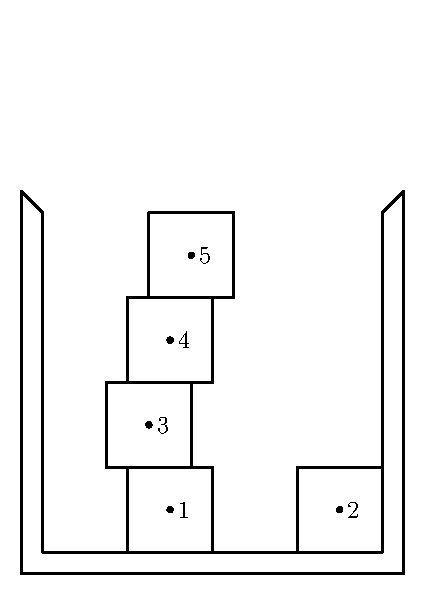
\includegraphics[height=\h]{btr-0}}%
\only<2>{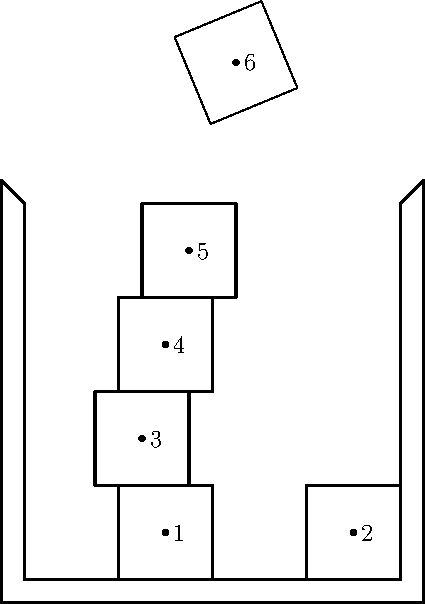
\includegraphics[height=\h]{btr-1}}%
\only<3>{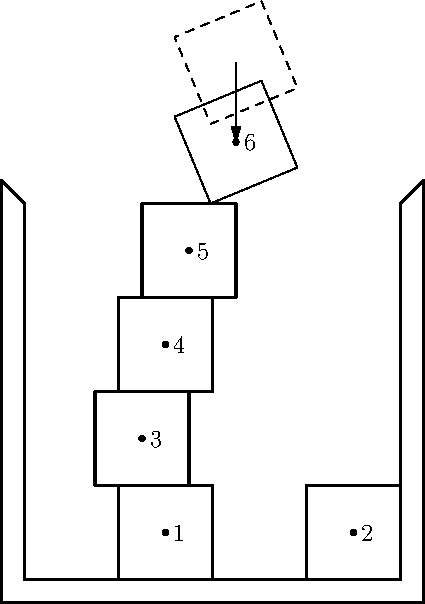
\includegraphics[height=\h]{btr-2}}%
\only<4>{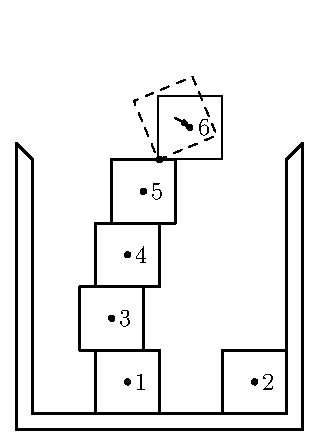
\includegraphics[height=\h]{btr-3}}%
\only<5>{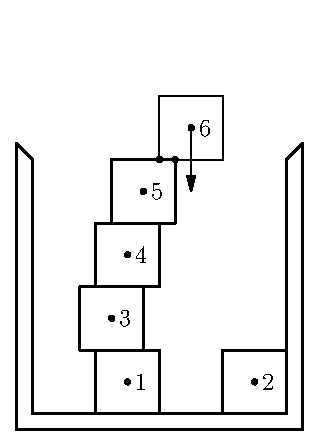
\includegraphics[height=\h]{btr-4}}%
\only<6>{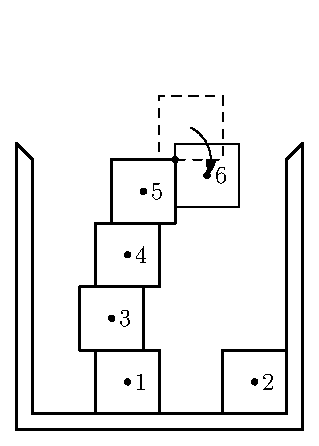
\includegraphics[height=\h]{btr-5}}%
\only<7>{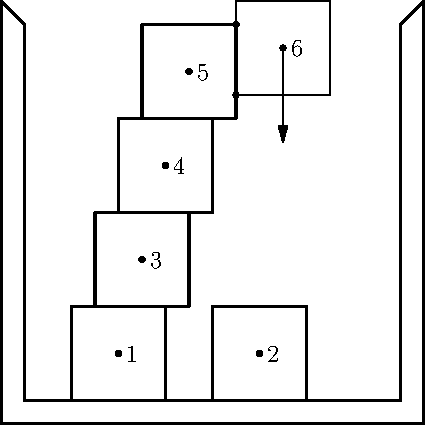
\includegraphics[height=\h]{btr-6}}%
\only<8>{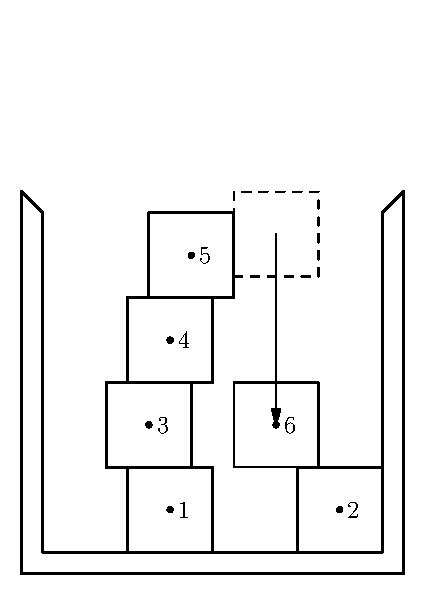
\includegraphics[height=\h]{btr-7}}%
\only<9>{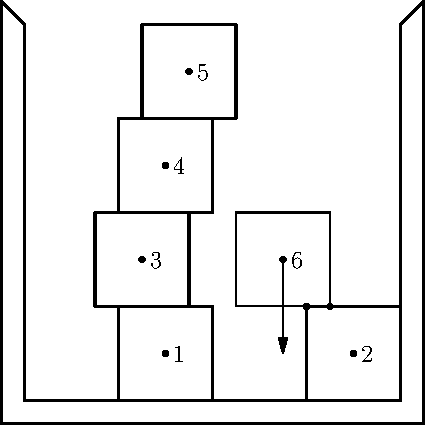
\includegraphics[height=\h]{btr-8}}%
\only<10>{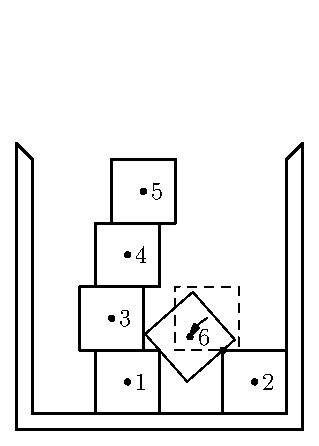
\includegraphics[height=\h]{btr-9}}%
\only<11>{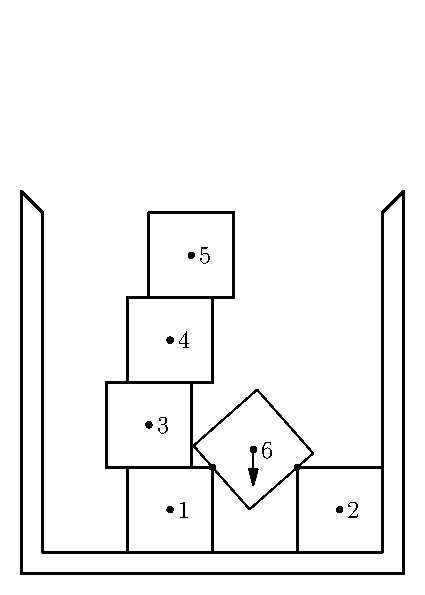
\includegraphics[height=\h]{btr-10}}%
\only<12>{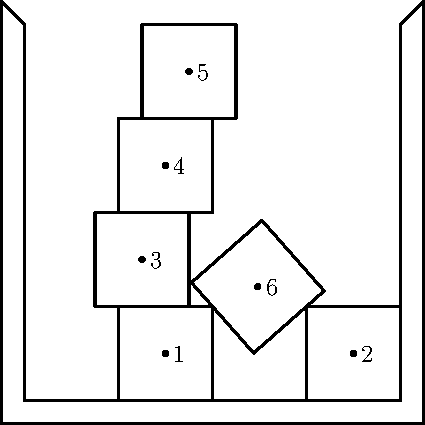
\includegraphics[height=\h]{btr-11}}
\end{block}
\end{frame}

\begin{frame}
\frametitle{Analysis}
\begin{block}{Packing Density}
We measured the packing density
\begin{align*}
\Delta & = \frac 1 V \sum_{i = 1}^N v_i,
\end{align*}
where $V$ is the volume of the container,
$N$ is the number of objects and
$v_i$ is the volume of the object $i$.
\end{block}
\end{frame}

\begin{frame}
\frametitle{Analysis}
\begin{block}{Randomness}
We also attempted to measure randomness.
Since the objects were not spherical,
it was difficult to find a suitable order metric.
We settled with the orientational correlation function
\begin{align*}
g & = \frac{\sum_{i = 1}^N \sum_{j = i + 1}^N (|\vec x_j - \vec x_i| < r) \max_{k, l} \cos 4 \arccos (\vec n_{i, k} \cdot \vec n_{j, l})}
{\sum_{i = 1}^N \sum_{j = i + 1}^N (|\vec x_j - \vec x_i| < r)},
\end{align*}
where $r$ is the nearest-neighbor range and
$\vec n_{i, k}$ is the $k$th surface normal of the object $i$.
The magic number $4$ comes from the size of the rotational symmetry group of the square.
\end{block}
\end{frame}

\begin{frame}
\frametitle{References}
\printbibliography
\end{frame}

\end{document}
